\documentclass{article}
\begin{article}
    Authorship Attribution using LLMs \\
Team GVMT - Gabriel Marx, Vy Dinh, Mark Peschel, and Tyler Lindsay \\
COMPSC 445: Machine Learning in Applied Data Science. \\
Abstract \\

Briefly write a summary of your work. You have to write it in three
parts in a single paragraph. First, discuss the background of the prob-
lem. Second, what you have done in the project; third, briefly write the
results/outcome of your project. (10 percents)

Authorship attribution is the problem of identifying who wrote a document.
In this project, we propose a method of attributing authorship using bigram language models,
which are normally used to generate the next token in a sequence of tokens. We trained a model on each author,
and then compared each model's probability of generating the text in question.
We found that this method of authorship attribution was competitive with (x, y, z) but worse than (a, b, c).


1 Introduction \\
The introduction will be a significant part of your project report. It will have
three paragraphs. In the first paragraph, you have to state what problem you
are solving. Provide a basic background of the problem. Why this problem is
important to solve, and what impact it might have. (5 percents)

Authorship attribution is the problem of identifying who wrote a document.
For example, the Federalist papers were known to be written by Alexander Hamilton, James Madison, and John Jay.
Twelve of the essays have disputed authorship.
In this case, authorship attribution can be used to analyse the text of an essay and guess which of the three wrote it.
Another example is the discovery of new works attributed to deceased authors.
In November 1985, a poem was discovered that was attributed to Shakespeare.
Authorship attribution could be used to determine if it was actually plausible for Shakespeare to write it.
Authorship attribution is important to solve because it can answer questions about who did what historically.
It can also verify whether newly discovered manuscripts are likely to have been written by authors to whom they are attributed.


In the second paragraph, you provide a literature review of the work. What
are similar works? Here you have to comment on their effectiveness in solving
the same problem. Try to tell about the strengths and limitations of their work.
You have to find out at least three relevant work of your problem. And must
cite them. Example of citation [1] [2] [3] [4]. (5 percents)

For the Federalist papers, Bosch and Smith (1998) found that 56 papers known to be written by Hamilton and 50 papers known to be written by Madison
could be separated by treating each paper as a vector of the frequencies of its words,
then finding a separating hyperplane based on the words "are", "our", and "upon".
This method was used to classify the twelve disputed Federalist papers as being probably Madison's work. [^7]
Bosch and Smith's results corroborate with preceding work by Mosteller, Wallace, & Nerbonne (1964) [^8].
For the 1985 Shakespeare poem, Thisted and Efron (1986) found that the frequencies of words in the poem, including new words not seen elsewhere,
was within tolerance for other works known to be written by Shakespeare. [^9]
However, there is a problem of comparing these techniques to each other; the datasets involved are large and varied.
Therefore, Gungor (2018) [^10] produced a standard dataset for benchmarking authorship attribution techniques.
He acquired 93 million words of text from 50 authors using the GDELT project.
He then cleaned and preprocessed this data and published it so future authorship attribution research could test their techniques against it.
He also tested a number of existing classification techniques,
including Naive Bayes Classifier, Support Vector Machines, k-means clustering, and more, to features derived from the texts, and evaluated them.
He found that SVMs on Bag-of-Words performed the best with f1 score of 0.73 of identifying the author of unknown texts,
even compared to sophisticated semantic approaches.


In the third paragraph, you establish why your work is important. Referring
to the second paragraph where you have discussed the literature of the work,
here you have to justify the need for your own work. (5 percents)

Since 2018, advances have been made in neural networks. Thanks to Gungor's work, it is possible to compare modern methods with
the state of the art 6 years ago. We propose a novel method of classifying text using the transformer architecture.
Specifically, we will attempt to use the same advances that have enabled ChatGPT to classify text.
We will then evaluate our model on Gungor's testing set using the f1 metric, demonstrating the utility of our method.


1.1 Our Contribution
In this section you use bullet points or enumerations to say what are the basic contributions of your project.
You may also write down the contribution of each team members.
(5 percents)

* Implemented a model-generation algorithm for producing recognizing models for an author from their body of work.
* Instantiated models for each of the 45 authors described in the dataset by Gungor.
* Developed a solution for assigning authorship to text based on probability-of-generation.
* Evaluated a novel method of authorship attribution by f1 score.
* Utilized f1 scores to compare the novel method of authorship attribution to existing methods.


2 Material and Methods
First, provide a block diagram of your work showing a graphical description of
your work. You have to describe the figure here. (5 percents)

\begin{figure}[h]
    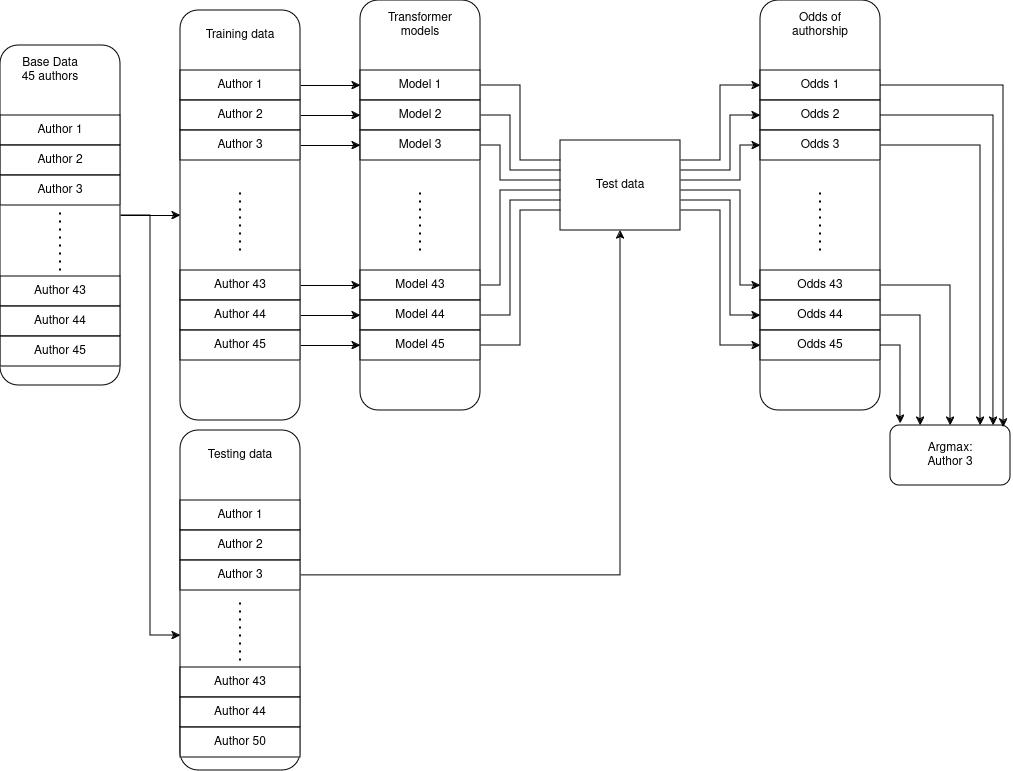
\includegraphics[width=\linewidth]{block_diagram.png}
\end{figure}

We begin with the preprocessed texts written by the fifty authors from the GDELT dataset.
This data has been split into training and testing sets for us. Five of the authors have been
removed entirely from the training set and exist only in the testing set; these authors make up \%34 of the testing data.
It is therefore impossible to get better than \%66 accuracy with a model that cannot recognize "unknown" authors.

After the data is divided into training and testing data, the training data is used to construct 45 "recognizer"
language models which each specialize in their specific author.
These models are then weighted based on how confident they are in recognizing their own training works.

For evaluation, the models are each given the feature data to classify.
Each model produces a confidence score based on the likelihood of each token given its subset context.
The model with the highest confidence is selected as the classification author.


2.1 Dataset Description 
Describe the datasets that you have used/collected. You must provide url /
citations to the dataset if not collected by you. Use a table to show the properties
or distributions of the dataset. If you have collected your own dataset, you must
put it in a GitHub repository and put the link in this section. If required, put
histograms, density distribution, or samples from your data here; also, state
why you have chosen the data. Describe all the features.
What are the attributes/ features (explain them)? What is/ are the tar-
get variable(s). Using domain specific knowledge, explain why you chose the
features. Describe the size of your dataset, its source and age.(10 percents)

Our dataset is the "Victorian Era Authorship Attribution" dataset collected by Abdulmecit Gungor and distributed at https://archive.ics.uci.edu/dataset/454/victorian+era+authorship+attribution
\begin{figure}[h]
    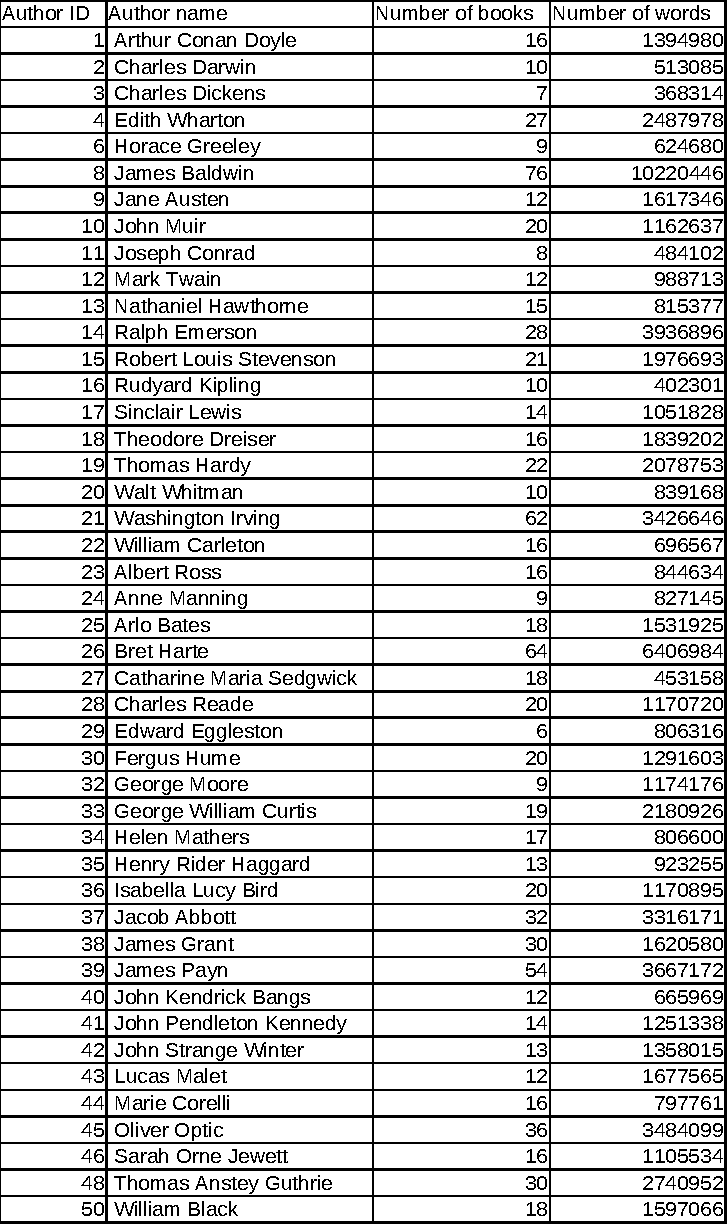
\includegraphics[width=\linewidth]{author_table.pdf}
\end{figure}



2.2 Algorithms Used or Methodology
Describe the details of the models or architectures that you have used. You have
to use multiple models. For each model, you may draw the separate diagrams
(depending on your project) and describe them in the text. Why have you
chosen them? What were the parameters and hyperparameters that you have
used? Why have you used them?
Also provide the Github link, colab link, or provide codes (as a attached file)
for your project(10 percents)
2.3 Performance Evaluation
Here, you have to state the function or metrics [2] [5] [6] you have used and how
you divided the dataset for training, validation, and test purpose.(5 percents)
3 Experimental Analysis
Here provide tables and graphs and describe them. There must be results with
multiple values or a set of values of the hyper-parameters for each model. You
need to compare the results in this section. Also, show convergence graphs (if
possible) for the train, validation/test sets. The link to the code in colab /
GitHub must be here.(15 points)
4 Conclusion
In this section you must again summarize your work. Tell about the limitations
and possible future work. (5 points)
5 Presentation
You need to present the project/research during the specified time. I will talk
about that during the class (20 percents)
2
6 For Master’s/ Ph.D student
Master’s or Ph.D students can submit a report similar to the IEEE/ACM paper
format or identical to the other journal’s layout.
References
[1] Peter Harrington. Machine learning in action (vol. 5). Greenwich, CT:
Manning, 2012.
[2] Md Faisal Kabir and Simone A Ludwig. Enhancing the performance of
classification using super learning. Data-Enabled Discovery and Applications,
3(1):5, 2019.
[3] Ashraful Haque, Jessica Engel, Sarah A Teichmann, and Tapio L¨onnberg.
A practical guide to single-cell rna-sequencing for biomedical research and
clinical applications. Genome medicine, 9(1):1–12, 2017.
[4] Malte D Luecken and Fabian J Theis. Current best practices in single-cell
rna-seq analysis: a tutorial. Molecular systems biology, 15(6):e8746, 2019.
[5] Md Faisal Kabir and Simone A Ludwig. Classification models and survival
analysis for prostate cancer using rna sequencing and clinical data. In 2019
IEEE International Conference on Big Data (Big Data), pages 2736–2745.
IEEE, 2019.
[6] Md Faisal Kabir, Tianjie Chen, and Simone A Ludwig. A performance
analysis of dimensionality reduction algorithms in machine learning models
for cancer prediction. Healthcare Analytics, 3:100125, 2023.
3

[7] 
Bosch, R. A., & Smith, J. A. (1998). Separating Hyperplanes and the Authorship of the Disputed Federalist Papers. The American Mathematical Monthly, 105(7), 601–608. https://doi.org/10.1080/00029890.1998.12004933
https://www.tandfonline.com/doi/abs/10.1080/00029890.1998.12004933

[8]
Mosteller, F., Wallace, D. L., & Nerbonne, J. A. (1964). Inference and disputed authorship: The Federalist. (No Title).

[9]
THISTED, R., & EFRON, B. (1986). 6 SSTSS.

[10]
Gungor, A. (2018). Benchmarking authorship attribution techniques using over a thousand books by fifty victorian era novelists (Doctoral dissertation, Purdue University).


\end{article}
